%\begin{sidewaysfigure}
%  \begin{center}
%  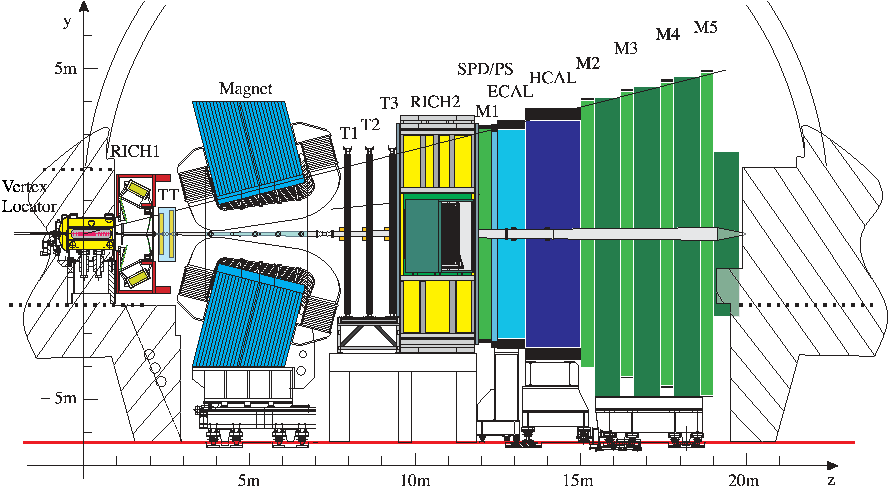
\includegraphics[width=0.8\textheight]{lhcb-detector-cross-section}
%  \caption[Cross-section view of \LHCb, cut in the non-bending $y$--$z$ plane]%
%    {Cross-section view of \LHCb, cut in the non-bending $y$--$z$ plane.}
%  \label{fig:LHCbCrossSection}
%  \end{center}
%\end{sidewaysfigure}



\chapter{Discussion and conclusions}
\label{chap:DiscussionAndConclusions}

\section{Discussion}
\label{sec:Discussion}
The results presented in chapter~\ref{chap:CrossSectionMeasurement} have potentially highlighted areas for improvement in the ND280 simulation.  Fig.~\ref{fig:MCTemplatesWithSystematicsT2KDataPreFit} showed discrepancies between data and MC for each ECal sample which ultimately led to the failure of the ECal rate fit when applied to T2K data.  Upon further inspection of the fit, it was noted that there were two significant areas of discrepancy between data and MC (shown in Fig.~\ref{fig:ClusterNHitsCutLevelGT0}).
\newline
\newline
As already discussed in chapter~\ref{chap:CrossSectionMeasurement}, one of the discrepancies appears to be correlated with the sand MC.  The sand MC is a relatively new addition to the ND280 simulation and has been tuned to tracker region data.  In most tracker analyses, the number of sand events which make it into the final selection generally number below 10 and so it is an area which has not required in depth study.  This is obviously not the case for ECal based analyses which see a much higher number of events originating from the surrounding pit.  The second discrepancy identified showed an excess of data events with a low number of hits in the reconstructed ECal clusters.  A brief study of such events suggests that they originate from the surrounding magnet region.  What is most troubling about these two issues is that they appear in the analysis at all.  Both topologies appear to be an entering background which strongly suggests that further study of the ECal fiducial volume is needed.  
\newline
\newline
As a separate problem, the reverse selection itself should be revisited.  This selection is currently defined as any event which passes the fiducial volume cut but fails the final (most upstream) cut.  While this allowed a large number of events to be included in the analysis, it also open up the possibility of data and MC mismodelling which either increases the systematic uncertainty or, like in this analysis, causes major issues in the final measurement.
\newline
\newline
However, this analysis has provided several important contributions to the T2K experiment.  The first is that the ECal is capable of reconstructing topologies outside of the single track or single shower hypotheses.  This is a potentially important milestone for the ECal as a neutrino detector as it paves the way for reconstructing neutrino events where the ECal is the active target.  The second contribution is that it is possible to apply a selection to the enhanced reconstruction to actually select neutrino interactions in the ECal.  While these developments have been used in a cross-section measurement, they were in no way developed solely with this analysis in mind.  So, the cross-section measurement itself can essentially be thought of as a by-product of the development of the reconstruction and selection.

\section{Conclusions}
\label{sec:Conclusions}
As highlighted in chapter~\ref{chap:Introduction}, the field of neutrino physics has rapidly evolved since the neutrino's discovery.  At time of writing, current and future generation neutrino oscillation experiments are aiming towards a measurements of the mass-hierarchy and the CP violating phase $\delta$.  To do this, a solid understanding of neutrino cross-section physics with atomic nuclei is vital. 
\newline
\newline
The overall aim of this analysis was to study neutrino interactions in the ND280 ECals, with a measurement of the $\nu_\mu$ CC inclusive cross-section on lead as the final goal.  To realise this, a new set of reconstruction algorithms were developed to allow the reconstruction of the charged final-states of the neutrino interactions in the ECal.  The output of this reconstruction was then used as the foundation of a $\nu_\mu$ CC inclusive selection which achieved a good efficiency and purity for both the barrel ECals and DS-ECal.  The final stage of the analysis was to use the selected events in a $\chi^2$ fit to extract the data-constrained rate of neutrino interactions on lead.  An important input to the fit itself was the evaluation of systematic uncertainties.  This involved a set of ECal systematic uncertainties which were evaluated for the first time and should be extremely useful to future analysers.
\newline
\newline
Unfortunately, there were unforeseen discrepancies between data and MC which caused major problems in the final fit.  These were overcome by introducing an ad hoc uncertainty which encompassed the migration of problematic background events between the signal enhanced and background enhanced samples.  With the inclusion of this extra uncertainty, the T2K flux-averaged $\nu_\mu$ charged current cross-section on lead was measured to be 
\begin{equation}
\langle \sigma^{\textrm{CC}}_{\textrm{Pb}} \rangle_{\phi} = 8.13^{+1.33}_{-1.26} \times 10^{-39} \textrm{ cm}^2 \textrm{ nucleon}^{-1}.
\end{equation}

\section{The future}
\label{sec:TheFuture}
The highest priority for future iterations of this analysis should be an in depth analysis of the problematic background events shown in Fig.~\ref{fig:ClusterNHitsCutLevelGT0}.  There are a few routes to take with such events but the general aim should be to either cut the events away in the selection and/or make improvements to the simulation itself.
\newline
\newline
There is an immense amount of scope for the reconstruction algorithms.  While the Hough transform has shown itself to be a very powerful method of reconstruction, analysis of the generated parameter space is actually very rudimentary.  As a reminder, the current method looks for the maxima in the parameter space which actually represent the 2D lines which pass through the most hits.  This analysis method needs improvement.  For example, the hits which are selected as constituents of the track are removed from the parameter space which means any subsequent track does not have that information available.  A more advanced method of hit masking would allow hit sharing between tracks to take place.  
\newline
\newline
Improvements can also be made to the selection.  As it stands, the selection does not fully harness the power of the enhanced reconstruction.  For example, particle identification could be applied to the individual tracks which would potentially allow removal of intrinsic background.
\newline
\newline
Most importantly, the reconstruction and selection provide much scope for expanding this analysis far beyond what is presented.  At the time of writing, a dedicated group of analyser is being set up with a common aim of studying neutrino interactions in the ECal and its potential for physics contributions.  For example, using the $\nu_\mu$ interaction rates in the barrel ECals to help constrain the flux in the ND280 tracker region and matching reconstructed ECal tracks to TPC tracks to make a $\nu_\mu$ CC differential cross-section measurement on lead.
\newline
\newline
Despite the large issues raised here, the main contribution of this analysis is that the many tools developed here pave the way for a wide range of neutrino interaction studies in which the ECal is the target.







